\documentclass[10pt]{beamer}
\usepackage{amsmath}
\usepackage{amssymb}
\usepackage{geometry}
\usepackage{graphicx}
\usepackage{url}
\usepackage{bm}

\makeatletter
\let \@sverbatim \@verbatim
\def \@verbatim {\@sverbatim \verbatimplus}
{\catcode`'=13 \gdef \verbatimplus{\catcode`'=13 \chardef '=13 }} 
\makeatother

\begin{document}

\begin{frame}
\large
Lecture 7:\\ 
Multiple Linear Regression\\
STAT 632, Spring 2020\\
\end{frame}

\begin{frame}{Polynomial Regression Example: Salary Data Set}
\begin{itemize}
\item For this example we consider a salary data set with $n=143$ observations and two variables.\footnote{\small Data set from ``A Modern Approach to Regression with R"}
\vspace{10pt}
\item We want to develop a regression model between $Y$, salary (in thousands of dollars), and $x$, the number of years of experience.  We are interested in using the model to make predictions and prediction intervals.
\vspace{10pt}
\item Since the variables have an obvious nonlinear, quadratic association we consider a polynomial regression model.
\end{itemize}
\end{frame}

\begin{frame}[fragile]{Polynomial Regression Example}
\scriptsize
\begin{verbatim}
> profsalary <- read.csv("https://ericwfox.github.io/data/profsalary.csv")
> lm1 <- lm(Salary ~ Experience, data=profsalary)
> plot(Salary ~ Experience, data=profsalary, 
       ylab='Salary', xlab='Years of Experience')
> abline(lm1)
\end{verbatim}
\begin{figure}
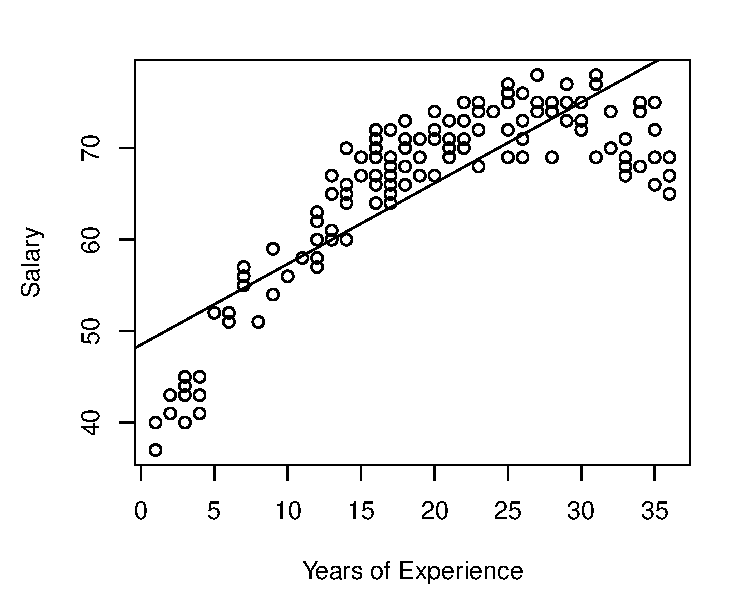
\includegraphics[scale=0.5]{figure/salary_plot1.pdf}
\end{figure}
\end{frame}

\begin{frame}[fragile]{Polynomial Regression Example}
\small
\begin{verbatim}
> plot(profsalary$Experience, resid(lm1), 
       xlab='Years of Experience', ylab='Residuals')
> abline(h=0)
\end{verbatim}
\begin{figure}
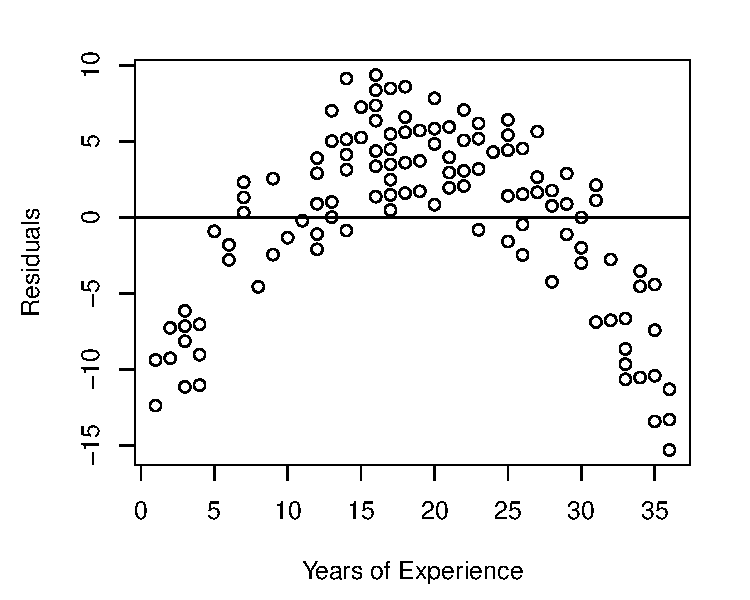
\includegraphics[scale=0.5]{figure/salary_resid1.pdf}
\end{figure}
\end{frame}

\begin{frame}[fragile]{Polynomial Regression Example}
Since a quadratic relationship is evident, we consider the following polynomial regression model:
$$Y = \beta_0 + \beta_1 x + \beta_2 x^2 + e$$
where $Y = $ salary, $x = $ years of experience, and $e \sim N(0, \sigma^2)$ is the random error.
\end{frame}

\begin{frame}[fragile]{Polynomial Regression Example}
\small
\begin{verbatim}
> lm2 <- lm(Salary ~ Experience + I(Experience^2), data=profsalary)
> summary(lm2)

Coefficients:
                 Estimate Std. Error t value Pr(>|t|)    
(Intercept)     34.720498   0.828724   41.90   <2e-16 ***
Experience       2.872275   0.095697   30.01   <2e-16 ***
I(Experience^2) -0.053316   0.002477  -21.53   <2e-16 ***
---
Signif. codes:  0 ‘***’ 0.001 ‘**’ 0.01 ‘*’ 0.05 ‘.’ 0.1 ‘ ’ 1

Residual standard error: 2.817 on 140 degrees of freedom
Multiple R-squared:  0.9247,	Adjusted R-squared:  0.9236 
F-statistic: 859.3 on 2 and 140 DF,  p-value: < 2.2e-16
\end{verbatim}
\end{frame}

\begin{frame}[fragile]{Polynomial Regression Example}
\small
\begin{verbatim}
plot(profsalary$Experience, resid(lm2), 
     xlab='Years of Experience', ylab='Residuals')
\end{verbatim}
\begin{figure}
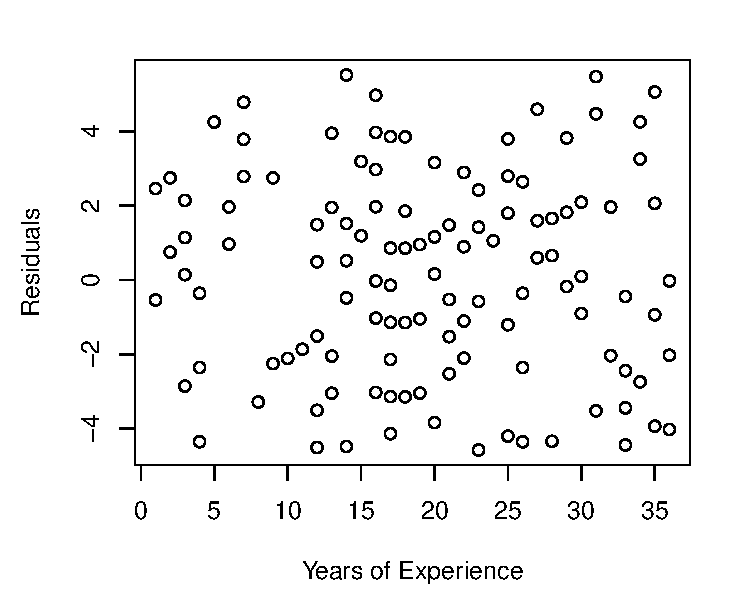
\includegraphics[scale=0.5]{figure/salary_resid2.pdf}
\end{figure}
\end{frame}

\begin{frame}[fragile]{Polynomial Regression Example}
Fitted regression model:
$$\hat{y} = 34.720 + 2.872x - 0.053x^2 $$
Prediction when $x=10$:
$$\hat{y} = 34.720 + 2.872(10) - 0.053(10^2) = 58.14$$\\
\vspace{5pt}

Using R:
\begin{verbatim}
> x_new <- data.frame(Experience = 10)
> predict(lm2, newdata=x_new, interval="prediction")
       fit      lwr      upr
1 58.11164 52.50481 63.71847
\end{verbatim}
\end{frame}

\begin{frame}{Polynomial Regression Example}
Add fitted quadratic curve to scatterplot.
\begin{figure}
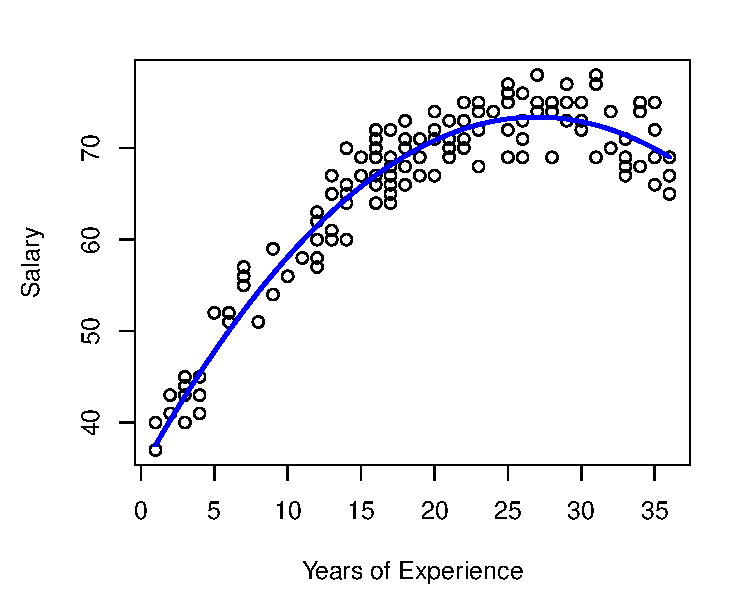
\includegraphics[scale=0.6]{figure/salary_polypred.pdf}
\end{figure}
\end{frame}

\begin{frame}[fragile]
Code used for last plot:
\begin{verbatim}
> range(profsalary$Experience)
[1]  1 36
> x_grd <- seq(1, 36, by=0.5)
> x_new <- data.frame(Experience = x_grd)
> preds <- predict(lm2, newdata = x_new)

> plot(Salary ~ Experience, data=profsalary, 
       ylab='Salary', xlab='Years of Experience')
> lines(x_grd, preds, col='blue', lwd=2.5)
\end{verbatim}
\end{frame}

\begin{frame}[fragile]
\begin{verbatim}
library(ggplot2)
ggplot(data=profsalary, aes(Experience, Salary)) +
  geom_point() +
  stat_smooth(method='lm', formula = y ~ poly(x, 2)) 
\end{verbatim}
\begin{figure}
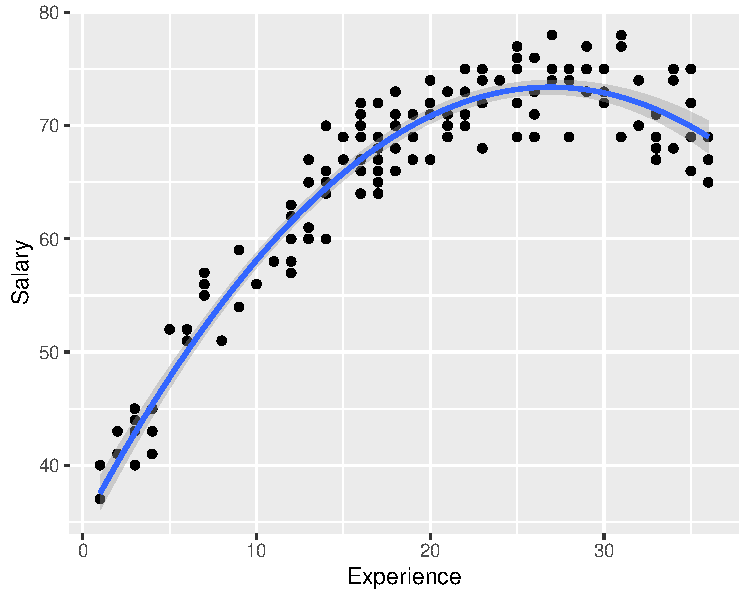
\includegraphics[scale=0.5]{figure/salary_polypred2.pdf}
\end{figure}
\end{frame}

\begin{frame}{Multiple Linear Regression (MLR) Model}
Suppose $Y$ is a response variable, and $x_1, \cdots, x_p$ are $p$ explanatory variables.  Then, the multiple linear regression model can be written as
$$Y = \beta_0 + \beta_1 x_1 + \beta_2 x_2 + \cdots + \beta_p x_p + e$$
where $e \sim N(0,\sigma^2)$ is the random error term.\\
\vspace{20pt}

For the polynomial regression example:\\
\begin{itemize}
\item $Y=$ salary
\item $x_1 = x$, years of experience
\item $x_2 = x^2$, (years of experience)$^2$
\end{itemize}
\end{frame}

%--------------------------------------------------------
\begin{frame}{Multiple Linear Regression (MLR) Model}
Suppose we have a collection $i=1,\cdots,n$ observations.  Then the multiple linear regression model for case $i$ is written as
$$Y_i = \beta_0 + \beta_1 x_{i1} + \beta_2 x_{i2} \cdots + \beta_p x_{ip} + e_i$$\\
where $e_i \sim N(0, \sigma^2)$ independently.
\vspace{15pt}

Given estimates $\hat{\beta}_0, \hat{\beta}_1, \cdots, \hat{\beta}_p$ of the parameters:
\begin{itemize}
\item The $i^{th}$ fitted (or predicted) value:
$$\hat{y}_i = \hat{\beta}_0 + \hat{\beta}_1 x_{i1} + \hat{\beta}_2 x_{i2} + \cdots + \hat{\beta}_p x_{ip}$$
\item The $i^{th}$ residual:
$$\hat{e}_i = y_i-\hat{y}_i = y_i - \hat{\beta}_0 - \hat{\beta}_1 x_{i1} - \hat{\beta}_2 x_{i2} - \cdots - \hat{\beta}_p x_{ip}$$
\end{itemize}
\end{frame}

\begin{frame}{Least Squares Estimation}
The parameters estimates $\hat{\beta}_0, \hat{\beta}_1, \hat{\beta}_2, \cdots, \hat{\beta}_p$ can be found by minimizing the sum of squared residuals:
\begin{align*}
&RSS = \sum_{i=1}^n (y_i - \hat{\beta}_0 - \hat{\beta}_1 x_{i1} - \hat{\beta}_2 x_{i2} - \cdots - \hat{\beta}_p x_{ip})^2
\end{align*}
\end{frame}
% remark the p is the number of predictors
% so there are (p+1) parameters (including the intercept)

\begin{frame}
To minimize set the partial derivatives equal to zero:
\begin{align*}
\frac{\partial RSS}{\partial \hat{\beta}_0} &= -2 \sum_{i=1}^n (y_i - \hat{\beta}_0 - \hat{\beta}_1 x_{i1} - \hat{\beta}_2 x_{i2} - \cdots - \hat{\beta}_p x_{ip}) = 0\\
\frac{\partial RSS}{\partial \hat{\beta}_1} &= -2 \sum_{i=1}^n x_{i1} (y_i - \hat{\beta}_0 - \hat{\beta}_1 x_{i1} - \hat{\beta}_2 x_{i2} - \cdots - \hat{\beta}_p x_{ip}) = 0\\
\vdots\\
\frac{\partial RSS}{\partial \hat{\beta}_p} &= -2 \sum_{i=1}^n x_{ip} (y_i - \hat{\beta}_0 - \hat{\beta}_1 x_{i1} - \hat{\beta}_2 x_{i2} - \cdots - \hat{\beta}_p x_{ip}) = 0\\
\end{align*}
This gives a system of $(p+1)$ equations with $(p+1)$ unknowns, which can be solved (assuming $p<n$) to obtain the least squares estimates $\hat{\beta}_0, \hat{\beta}_1, \cdots, \hat{\beta}_p$.  In practice, we can use the \texttt{lm()} function in R to do these computations.    
\end{frame}

\begin{frame}
\begin{figure}
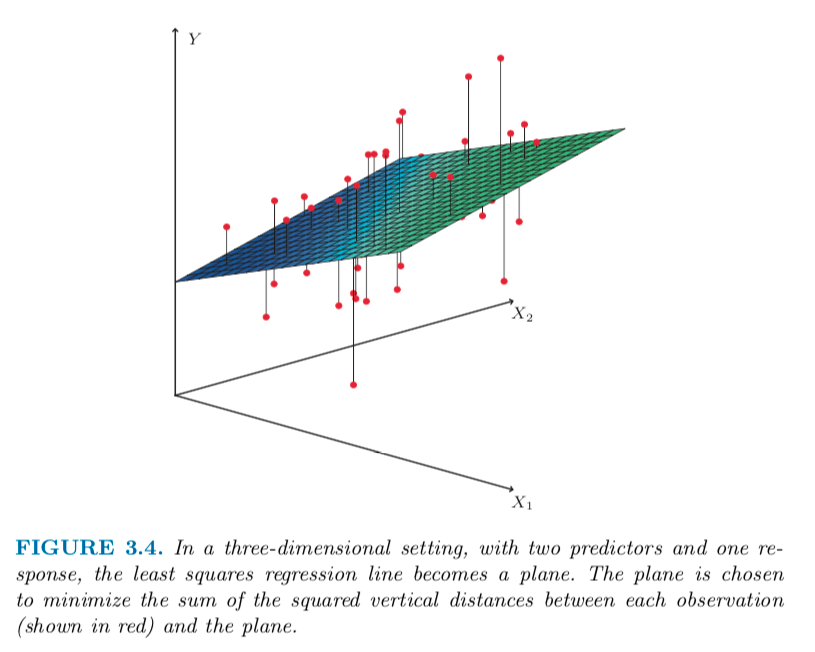
\includegraphics[scale=0.3]{figure/planeISLR.png}
\end{figure}
\scriptsize
From Chapter 3, p. 73, of \emph{An Introduction to Statistical Learning}.
\end{frame}

\begin{frame}{Estimating $\sigma^2$}
\begin{align*}
\hat{\sigma}^2 &= \frac{\text{RSS}}{n-p-1} = \frac{1}{n-p-1} \sum_{i=1}^n (y_i - \hat{y}_i)^2\\
&= \frac{1}{n-p-1} \sum_{i=1}^n (y_i - \hat{\beta}_0 - \hat{\beta}_1 x_{i1} - \hat{\beta}_2 x_{i2} -  \cdots - \hat{\beta}_p x_{ip})^2 
\end{align*}
\begin{itemize}
\item $\hat{\sigma} = \sqrt{\text{RSS} / (n-p-1)}$ is the residual standard error.
\vspace{5pt}
\item It can be shown that $\hat{\sigma}^2$ is an unbiased estimate of $\sigma^2$ (i.e., $E(\hat{\sigma}^2) = \sigma^2$).
\end{itemize}
\end{frame}

\begin{frame}{Hypothesis Test for a Single Predictor}
Test whether parameter $\beta_j$ is zero.\\
\vspace{10pt}

$H_0: \beta_j = 0$\\
$H_A: \beta_j \neq 0$\\
\vspace{10pt}

Test statistic:
$$ T_j = \frac{\hat{\beta}_j}{se(\hat{\beta}_j)}; \quad \text{df} = n-p-1 $$
\begin{itemize}
\item $se(\hat{\beta}_j)$ is the standard error of $\hat{\beta}_j$
\item $n$ is the number of observations
\item $p$ is the number of predictor variables
\item degrees of freedom (df) =\\ 
sample size - number of parameters estimated $= n - p-1$\\ 
(since, when including the intercept, there are $p+1$ parameters)
\end{itemize}
\end{frame}



\begin{frame}{Confidence Interval for a Single Predictor}
A $1-\alpha$ confidence interval for $\beta_j$:
$$ \hat{\beta}_j \pm t_{\alpha/2; n-p-1} se(\hat{\beta}_j) $$\\
\vspace{10pt}

The R function \texttt{confint()} can be used to calculate confidence intervals for the parameters.
\end{frame}

\begin{frame}{Coefficient of Determination ($R^2$)}
The coefficient of determination $R^2$ has the same definition for simple and multiple linear regression.
\begin{align*}
R^2 = \frac{\text{SSReg}}{\text{SST}} = 1 - \frac{\text{RSS}}{\text{SST}}
\end{align*}
\begin{itemize}
\item $SST = \sum_{i=1}^n (y_i - \bar{y})^2$ is the total sum of squares 
  \begin{itemize}
  \item total variability in the response variable
  \end{itemize}
\vspace{5pt}
\item $SSreg = \sum_{i=1}^n (\hat{y}_i - \bar{y})^2$ is the regression sum of squares
  \begin{itemize}
  \item variability in the response explained by the model
  \end{itemize}
\vspace{5pt}
\item $RSS = \sum_{i=1}^n (y_i - \hat{y}_i)^2$ is the residual sum of squares
  \begin{itemize}
  \item unexplained variability
  \end{itemize}
\end{itemize}
\end{frame}

\begin{frame}{Coefficient of Determination ($R^2$)}
\begin{align*}
R^2 = \frac{\text{SSReg}}{\text{SST}} = 1 - \frac{\text{RSS}}{\text{SST}}
\end{align*}
\begin{itemize}
\item $R^2$ can be interpreted as the proportion of variability in the response  $Y$ that is explained by the regression model.\\
\vspace{5pt}
\item $0 \leq R^2 \leq 1$, where values closer to 1 indicate a better linear fit to the data.\\
\vspace{5pt}
\item \textbf{Problem with $R^2$ in MLR}: Adding predictor variables to the regression model will always increases $R^2$ (or, equivalently decrease RSS).  Even if the predictor variable is irrelevant (noise) the $R^2$ will increase slightly.  This is not ideal since simpler models are preferred to more complicated models.
\end{itemize}
\end{frame}

\begin{frame}
\textbf{Occam's razor}, or the law of parsimony, is a problem solving principle that states that simpler solutions are preferred to more complex ones.\footnote{\url{https://en.wikipedia.org/wiki/Occam's_razor}}\\
\vspace{15pt}
``Everything should be kept as simple as possible, but not simpler" --Albert Einstein

\begin{figure}

\includegraphics[scale=0.3]{figure/ockham.png}
\hspace{2cm}
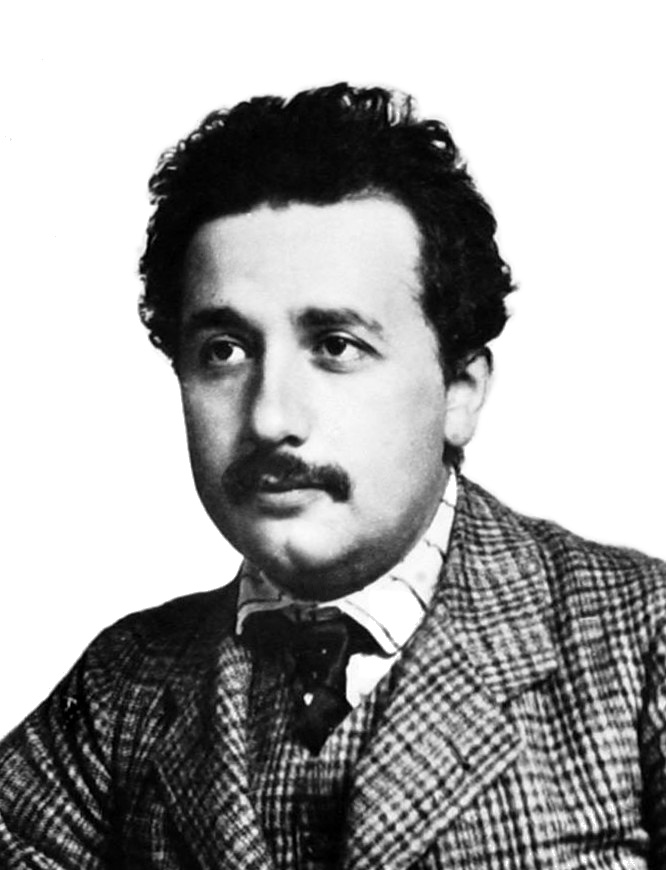
\includegraphics[scale=0.15]{figure/einstein.jpg}
\end{figure}
\end{frame}
% Ockham was a franciscian fryer
% ``shave away all but what is necessary"

\begin{frame}{Adjusted Coefficient of Determination ($R^2_{adj}$)}
$$R^2_{adj} = 1 - \frac{RSS / (n-p-1)}{SST/(n-1)}$$
\begin{itemize}
\item The denominator in RSS$/(n-p-1)$ penalizes for adding extra predictor variables.\\
\vspace{5pt}
\item The idea is that the $R^2_{adj}$ should decrease when adding an irrelevant predictor variables into a model.\\
\vspace{5pt}
\item When comparing models with different numbers of predictors one should use $R^2_{adj}$ and not $R^2$.
%\item While RSS will always decrease as the number of predictors $p$ increases, RSS$/(n-p-1)$ may either increase or decrease.\\
%\item The intuition is that adding irrelevant (noise) predictors will lead to an increase RSS$/(n-p-1)$ and therefore a decrease in $R^2_{adj}$.\\
%\item $R^2_{adj}$ should not be used to compare models with different transformations of the response variable.
\end{itemize}
\end{frame}


\begin{frame}{MLR Example: Menu Pricing Data Set}
Data set from surveys of customers of 168 Italian restaurants in New York City.\footnote{Zagat Survey 2001: New York City Restaurants} 
\vspace{10pt}

The variables are:
\begin{itemize}
\item $Y =$ Price = the price (in \$US) of dinner (including 1 drink and tip)
\item $x_1 =$ Food = customer rating of the food (out of 30)
\item $x_2 =$ Decor = customer rating of the decor (out of 30)
\item $x_3 =$ Service = customer rating of the service (out of 30)
\item $x_4 =$ East = dummy variable, 1 (0) if the restaurant is east (west) of Fifth Avenue
\end{itemize}
\end{frame}

\begin{frame}[fragile]{MLR Example: Menu Pricing Data Set}
\small
\begin{verbatim}
> nyc <- read.csv("https://ericwfox.github.io/data/nyc.csv")
> pairs(Price ~ Food + Decor + Service, data=nyc)
\end{verbatim}
\begin{figure}
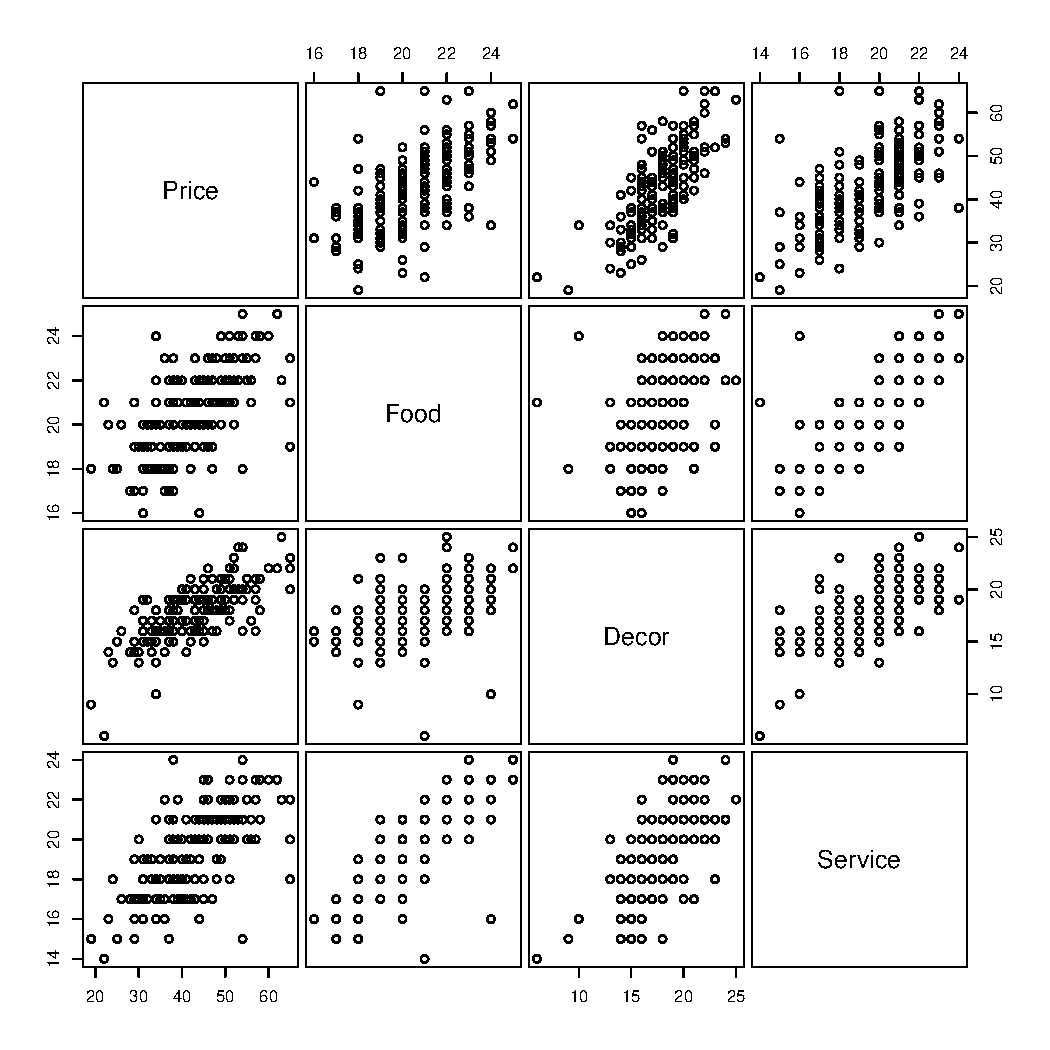
\includegraphics[scale=0.4]{figure/menu_pairs.pdf}
\end{figure}
\end{frame}

\begin{frame}[fragile]{MLR Example: Menu Pricing Data Set}
\small
\begin{verbatim}
> boxplot(Price ~ East, data= nyc, 
          ylab="Price", xlab="East (1 = East of Fifth Avenue)")
\end{verbatim}
\begin{figure}
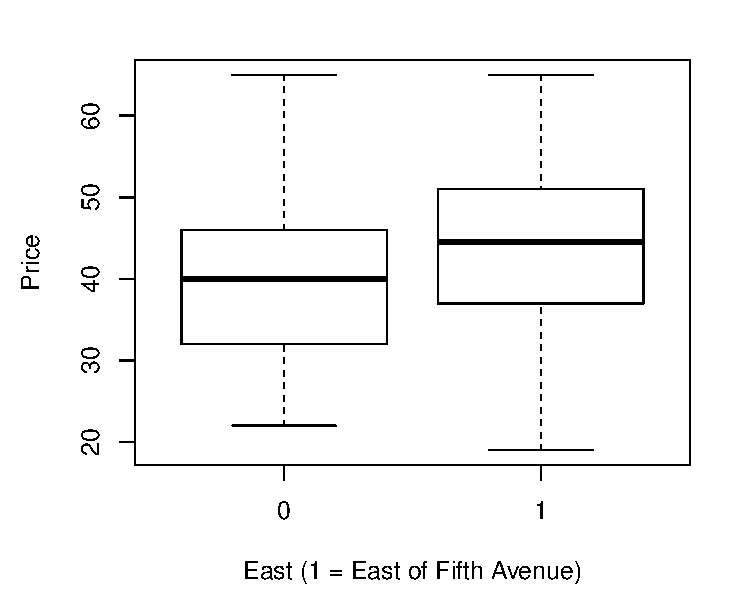
\includegraphics[scale=0.5]{figure/east_boxplot.pdf}
\end{figure}
\end{frame}

\begin{frame}[fragile]{MLR Example}
\small
\begin{verbatim}
> lm1 <- lm(Price ~ Food + Decor + Service + East, data=nyc)
> summary(lm1)

Coefficients:
              Estimate Std. Error t value Pr(>|t|)    
(Intercept) -24.023800   4.708359  -5.102 9.24e-07 ***
Food          1.538120   0.368951   4.169 4.96e-05 ***
Decor         1.910087   0.217005   8.802 1.87e-15 ***
Service      -0.002727   0.396232  -0.007   0.9945    
East          2.068050   0.946739   2.184   0.0304 *  
---
Signif. codes:  0 ‘***’ 0.001 ‘**’ 0.01 ‘*’ 0.05 ‘.’ 0.1 ‘ ’ 1

Residual standard error: 5.738 on 163 degrees of freedom
Multiple R-squared:  0.6279,	Adjusted R-squared:  0.6187 
F-statistic: 68.76 on 4 and 163 DF,  p-value: < 2.2e-16
\end{verbatim}
\end{frame}

\begin{frame}[fragile]{MLR Example}
Since \texttt{Service} is not significant we remove it from the model.
\small
\begin{verbatim}
> lm2 <- lm(Price ~ Food + Decor + East, data=nyc)
> summary(lm2)

Coefficients:
            Estimate Std. Error t value Pr(>|t|)    
(Intercept) -24.0269     4.6727  -5.142 7.67e-07 ***
Food          1.5363     0.2632   5.838 2.76e-08 ***
Decor         1.9094     0.1900  10.049  < 2e-16 ***
East          2.0670     0.9318   2.218   0.0279 *  
---
Signif. codes:  0 ‘***’ 0.001 ‘**’ 0.01 ‘*’ 0.05 ‘.’ 0.1 ‘ ’ 1

Residual standard error: 5.72 on 164 degrees of freedom
Multiple R-squared:  0.6279,	Adjusted R-squared:  0.6211 
F-statistic: 92.24 on 3 and 164 DF,  p-value: < 2.2e-16
\end{verbatim}
\end{frame}

\begin{frame}[fragile]
\small
\begin{verbatim}
> s1 <- summary(lm1)
> s2 <- summary(lm2)

> s1$r.squared
[1] 0.6278809
> s2$r.squared
[1] 0.6278808
 
> s1$adj.r.squared
[1] 0.6187492
> s2$adj.r.squared
[1] 0.6210738

#---------------------------------
> confint(lm2) 
                 2.5 %     97.5 %
(Intercept) -33.253364 -14.800395
Food          1.016695   2.055996
Decor         1.534181   2.284565
East          0.227114   3.906912
\end{verbatim}
\end{frame}

\begin{frame}[fragile]{MLR Example}
The final regression model is:\\
$$\widehat{\texttt{Price}} = -24.03 + 1.54 \texttt{Food} + 1.91 \texttt{Decor} + 2.07\texttt{East}$$ \\
\vspace{10pt}
For example, we can use the model to predict \texttt{Price} when \texttt{Food=20}, \texttt{Decor=16} and \texttt{East=1}:
$$\widehat{\texttt{Price}} = -24.03 + 1.54(20) + 1.91(16) + 2.07(1) = 39.4$$
We can also use R to make this prediction and to calculate a 95\% prediction interval.
\begin{verbatim}
> new_x <- data.frame(Food = 20, Decor = 16, East = 1)
> predict(lm2, newdata = new_x, interval="prediction")
       fit      lwr      upr
1 39.31701 27.95384 50.68019
\end{verbatim}
\end{frame}

\begin{frame}{MLR Example}
The final regression model is:\\
$$\widehat{\texttt{Price}} = -24.03 + 1.54 \texttt{Food} + 1.91 \texttt{Decor} + 2.07\texttt{East}$$ \\

\begin{itemize}
\item \texttt{Decor} has the largest effect on \texttt{Price} since its regression coefficient is largest.  Note that \texttt{Food}, \texttt{Decor}, and \texttt{Service} are on the same 0 to 30 scale, so it is meaningful to make the comparison.  
\vspace{10pt}
\item If a goal is to maximize \texttt{Price} for a new restaurant, it should be located east of Fifth Avenue (i.e., \texttt{East} = 1).
\end{itemize}
\end{frame}


\begin{frame}{Interpreting Regression Coefficients}
Suppose we fit a multiple linear regression model 
$$\hat{y} = \hat{\beta}_0 + \hat{\beta_1} x_1 + \hat{\beta}_2 x_2 + \cdots + \hat{\beta}_p x_p + e,$$
where $x_j$ is the $j^{th}$ predictor and $\hat{\beta}_j$ the estimated coefficient for the variable.\\
\vspace{15pt}

How do we interpret $\hat{\beta}_j$?\\
\vspace{5pt}
The usual interpretation is as follows: an increase in $x_j$ by 1, \emph{with all other predictors in the model held fixed}, is associated with a change of $\hat{\beta_j}$ in the predicted response, $\hat{y}$. 
\end{frame}

\begin{frame}{Interpreting Regression Coefficients}
Going back to the example, the final regression model is
$$\widehat{\texttt{Price}} = -24.03 + 1.54 \texttt{Food} + 1.91 \texttt{Decor} + 2.07\texttt{East}$$

\begin{itemize}
\item Interpret the coefficient for \texttt{Decor}: a one unit increase in the customer rating of decor, with the other predictors (\texttt{Food} and \texttt{East}) held fixed, is associated with an increase in \texttt{Price} by \$1.91.
\vspace{5pt}
\item Interpret the coefficient for the dummy variable \texttt{East}: the price of dinner at a restaurant east of Fifth Avenue will cost \$2.07 more, on average, than a restaurant west of Fifth Avenue, when all other predictors (\texttt{Food} and \texttt{Decor})  are held fixed.
\end{itemize}
\end{frame}
% Write this part on the board
% \begin{frame}{Interpreting Regression Coefficients}
% For example, we can quantify the effect \texttt{Decor} has on \texttt{Price} when \texttt{Food} equal to its sample mean (20.6) and \texttt{East} is equal 1 with the equation:
% \begin{align*}
% \widehat{\texttt{Price}} &= -24.03 + 1.54 (20.6) + 1.91 \texttt{Decor} + 2.07(1)\\
% &= 9.76 + 1.91 \texttt{Decor}
% \end{align*}
% Here we can clearly see that when we fix the values of the other predictors it only affects the intercept, not the slope.
% \end{frame}


\begin{frame}{Interpreting Regression Coefficients}
Some problems when interpreting regression coefficients:
\vspace{5pt}
\begin{itemize}
\item The interpretation of $\beta_j$ as the average change in $Y$ per unit change in $x_j$, \emph{with all other predictors held fixed}, assumes predictors can be changed without affecting other predictors.
\vspace{5pt}
\item Interpretation becomes hazardous when there are correlations amongst predictors.  When $x_j$ changes, then values for other predictors also change. 
\vspace{5pt}
\item The magnitude and sign of a coefficient can change when including (or removing) another predictor from the model.
\vspace{5pt}
\item For observational data we can only make claims about associations, not causation.
\end{itemize}
\end{frame}





\end{document}
